\documentclass[11pt]{scrartcl}


\usepackage[sexy]{evan}
\usepackage{import}
\usepackage[table]{xcolor}
\usepackage{xfp}

\newcommand{\gad}{\textcolor{yellow}{$\bigstar$}}
\newcommand{\bad}{\textcolor{red}{$\bigstar$}}

\definecolor{dcol0}{HTML}{C8E6C9}
\definecolor{dcol1}{HTML}{D4E9B3}
\definecolor{dcol2}{HTML}{E5ED9A}
\definecolor{dcol3}{HTML}{FFF59D}
\definecolor{dcol4}{HTML}{FFE082}
\definecolor{dcol5}{HTML}{FFCC80}
\definecolor{dcol6}{HTML}{FFAB91}
\definecolor{dcol7}{HTML}{F49890}
\definecolor{dcol8}{HTML}{E57373}
\definecolor{dcol9}{HTML}{D32F2F}

\makeatletter
\newcommand{\getcolorname}[1]{dcol#1}
\makeatother

\newcommand{\dif}[1]{%
    \edef\colorindex{\number\fpeval{floor(#1)}}%
    \edef\fulltext{#1}%
    \colorbox{\getcolorname{\colorindex}}{%
        \ifnum\colorindex>8
            \textbf{\textcolor{white}{\,\fulltext\,}}%
        \else
            \textbf{\textcolor{black}{\,\fulltext\,}}%
        \fi
    }%
}
% Variable para dificultad (inicial 0)
\newcommand{\thmdifficulty}{0}

% Comando para asignar dificultad antes del problema
\newcommand{\problemdiff}[1]{\renewcommand{\thmdifficulty}{#1}}

% Estilo del problema que incluye dificultad antes del título
\declaretheoremstyle[
    headfont=\color{blue!40!black}\normalfont\bfseries,
    headformat={%
      \dif{\thmdifficulty}\quad \NAME~\NUMBER\ifx\relax\EMPTY\relax\else\ \NOTE\fi
    },
    postheadspace=1em,
    spaceabove=8pt,
    spacebelow=8pt,
    bodyfont=\normalfont
]{problemstyle}

    \declaretheorem[style=problemstyle,name=Problema,sibling=theorem]{problema}
    \declaretheorem[style=problemstyle,name=Problema,numbered=no]{problema*}

\definecolor{yellow4}{RGB}{255, 206, 0}

\title {Conteo}

\author{Emma y Ale}


\begin{document}
\maketitle


\section{Problemas}
\epigraph{Cause I feel like I'm the worst\\
So I always act like I'm the best}{Oh No! - MARINA}



\problemdiff{2}
\begin{problem}
   % [OMMC 2021/4]
    Determina cuantas secuencias de números reales $a_1, a_2, \ldots, a_9$ cumplen
    \[|a_1-1|=|a_2-a_1|=\cdots=|a_9-a_8|=|1-a_9|=1\]
\end{problem}

\problemdiff{3}
\begin{problem}
   % [AIME II 2021/6]
    Encuentra el numero de pares ordenados $(A,B)$ de subconjuntos de $\{1,2,3,4,5,6,7,8\}$ que cumplen:
    $$|A| \cdot |B| = |A \cap B| \cdot |A \cup B|$$

    \textit{Nota: } $|A|$ es la cantidad de elementos de $A$.
\end{problem}

\problemdiff{3}
\begin{problem}
   % [ARML 2023 T-6]
    Lalo construye una tabla circular, en la cual escribe enteros positivos de forma que esten igualmente espaciados en la circunferencia. El considera dos tablas iguales si una puede ser rotada para obtener los mismos numeros en las mismas posiciones que la otra. Encuentra el numero de tablas distintas para las cuales la suma de sus enteros positivos es 17.
\end{problem}

\problemdiff{3}
\begin{problem}
    El país Olimpia esta formado por $n$ islas. La más poblada se llama Panacenter, y cada isla tiene un número diferente de habitantes. Queremos construir puentes entre estas islas , con las que podremos 
    viajar en ambas direcciones, bajo las siguientes condiciones: Ningún par de islas está unido por más de un puente. Utilizando
los puentes podemos llegar a todas las islas desde el Panacentro. Si queremos viajar desde Panacenter a cada
una de las otras islas, de forma que utilicemos cada puente como máximo una vez, el número de habitantes
de las islas que visitamos es estrictamente decreciente. \\
Determina el número de formas en que podemos construir los puentes.
\end{problem}

\problemdiff{3}
\begin{problem}
    Un tablero cuadrado con 8cm lados se divide en 64 casillas con cada lado 1cm. Cada casilla puede estar
pintada de blanco o de negro. Halla el número total de formas de colorear el tablero para que cada cuadrado
de lado 2cm formado por cuatro casillas con un vértice común contenga dos casillas blancas y dos negras.
\end{problem}

\problemdiff{3.5}
\begin{problem}
  %  [KJMO 2022/2]
    Para un entero positivo $n \geq 3$, encuentra el numero de secuencias de $n$ enteros $(a_1, a_2, \ldots, a_n )$ positivos tal que:
    \begin{itemize}
        \item Para todo entero positivo $1 \leq i \leq n$ se cumple que $1\leq a_i \leq  i$.
        \item Para enteros positivos $i,j,k$ con $1 \leq i <j <k \leq n$ si $a_i=a_j$ entonces $a_j \geq a_k$.
    \end{itemize}
\end{problem}


\problemdiff{4}
\begin{problem}
    Sea $n$ un entero positivo. Cada punto $(x,y)$ en el plano, donde $x$ e $y$ son enteros no negativos con $x+y < n$ esta coloreado de rojo o azul,
    sujeto a la siguiente condicion: si $(x,y)$ es un punto rojo, entonces tambien lo son todos los puntos $(x',y')$ con $x'\leq x, y'\leq y$. Sea $A$ el numero 
    de maneras de elegir $n$ puntos azules con coordenadas $x$ distintas, y sea $B$ el número de formas de elegir $n$ puntos azules con coordenadas $y$ distintas. Demuestra que $A=B$.
\end{problem}

\problemdiff{4}
\begin{problem}
%    [OMM 2015/2]
      Sea $n$ un entero positivo y $k$ un entero entre $1$ y $n$. Se tiene un tablero de $n \times n$ color blanco. Se hace el siguiente proceso. Se dibujan $k$ rectángulos con lados de longitud entera, con lados paralelos a los del tablero y tales que su esquina superior derecha coincide con la del tablero. Luego, estos $k$ rectángulos se rellenan de negro. Esto deja una figura blanca en el tablero.
¿Cuántas figuras blancas diferentes podemos obtener, que no se puedan obtener haciendo el proceso con menos de $k$ rectángulos?
\end{problem}

\problemdiff{4}
\begin{problem}
 %   [OMM 2006/3]
    Sea $n$ un número entero mayor que $1$. ¿De cuántas formas se pueden acomodar todos los números $1,2,3,\dots 2n$ en las casillas de una cuadrícula de $2\times n$, uno en cada casilla, de manera que cualesquiera dos números consecutivos se encuentren en casillas que comparten un lado en la cuadrícula?
\end{problem}

\problemdiff{4}
\begin{problem}
 %   [Canada 2019/3]
    Un tablero de $2m \times 2n$ es coloreado como ajedrez. Encuentra la forma de acomodar $mn$ tijeras en los cuadrados blancos, de tal forma que cada cuadrado contenga a lo más unas tijeras, y no hay dos cuadrados blancos adyacentes diagonalmente con tijeras. 
\end{problem}

\problemdiff{4.5}
\begin{problem}
%    [OMM 2021/3] 
    Sean $m,n\geq 2$ dos enteros. En una cuadrícula de $m\times n$, una hormiga empieza en el cuadrito inferior izquierdo y quiere caminar al camino superior derecho. Cada paso que da la hormiga debe ser a un cuadrito adyacente, y de acuerdo a las siguientes posibilidades: $\uparrow$, $\rightarrow$ y $\nearrow$. Sin embargo, un malvado mago ha dejado caer lava desde arriba de la cuadrícula y ha destruido algunos cuadritos, de forma tal que:
 \begin{itemize} 
 \item Si un cuadrito está destruido, entonces todos los cuadritos superiores a él también también están destruidos.

 \item El número de cuadritos destruidos es mayor o igual a $0$.

 \item Quedan suficientes cuadritos sin destruir para que la hormiga pueda llegar a la meta. 
 \end{itemize} 
Sea $P$ el número de caminos de longitud par que puede seguir la hormiga. Sea $I$ el número de caminos de longitud impar que puede seguir la hormiga. Encuentra todos los posibles valores de $P-I$.
    \begin{center}
        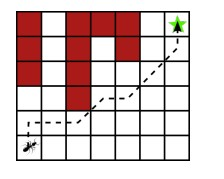
\includegraphics[scale=0.6]{21OMM3.jpg}
    \end{center}
\end{problem}

\problemdiff{5}
\begin{problem}
%[EGMO 2015/2]
    Una domino es una pieza de $1\times 2$ o $2\times 1$. Determina de cuantas formas puedes acomodar $n^2$ dominos sin que se encimen en un tablero de $2n \times 2n $, de forma que cada cuadrado de $2\times2$ contiene 2 cuadrados en la misma fila o columna que estan cubiertos por un domino.
\end{problem}


\problemdiff{5}
\begin{problem}
 %   [OMM 2025/3]
    Sea $n$ un entero positivo. Considera un tablero de $2\times n$ dividido en cuadrados de $1\times 1$. Cada uno de los cuadrados se etiquetan con un número distinto elegido de entre el $1$ al $2n$, utilizando cada número exactamente una vez.  \\
    Definimos un camino en una cuadricula etiquetada como una sucesión de cuadrados, de manera que cada par de cuadrados consecutivos comparten un lado de la cuadricula, y que nunca visita un cuadrado más de una vez. Un camino es ascendente si las etiquetas de los cuadrados visitados estan en orden creciente ( es decir, si el camino pasa por el cuadrado etiquetado $i$ y despues por el cuadrado etiquetado $j$, entonces $i<j$). 
    Por ultimo un camino es completo si inicia en el cuadrado etiquetado $1$ y termina en el cuadrado etiquetado $2n$. \\
    Para cada uno de los etiquetados del rectangulo $2\times n$ se calcula el número de caminos ascendentes completos. Determina el máximo de estos números en terminos de $n$. 
\end{problem}

\end{document}